\documentclass[12pt,a4paper]{report}

% ─── Packages ──────────────────────────────────────────────────────────────────
\usepackage[margin=2.5cm]{geometry}
\usepackage[T1]{fontenc}
\usepackage[utf8]{inputenc}
\usepackage{lmodern}
\usepackage{microtype}
\usepackage[dvipsnames]{xcolor}
\usepackage{listings}
\usepackage{minted}
\usepackage{graphicx}
\usepackage{tikz}
\usepackage{pgf-umlsd}
\usepackage{booktabs}
\usepackage{tabularx}
\usepackage{longtable}
\usepackage{enumitem}
\usepackage{hyperref}
\usepackage{tcolorbox}
\usepackage{fancyhdr}
\usepackage{titlesec}
\usepackage{parskip}
\usepackage{amsmath}
\usepackage{caption}
\usepackage{float}

\usetikzlibrary{arrows.meta, positioning, shapes.geometric, fit, backgrounds, calc}

% ─── Colours ───────────────────────────────────────────────────────────────────
\definecolor{safeblue}{RGB}{26,86,219}
\definecolor{safegreen}{RGB}{22,163,74}
\definecolor{safered}{RGB}{220,38,38}
\definecolor{safeyellow}{RGB}{202,138,4}
\definecolor{safegray}{RGB}{107,114,128}
\definecolor{codebg}{RGB}{248,248,248}
\definecolor{codeborder}{RGB}{221,221,221}

% ─── Hyperref ──────────────────────────────────────────────────────────────────
\hypersetup{
  colorlinks=true,
  linkcolor=safeblue,
  urlcolor=safeblue,
  citecolor=safeblue,
  pdftitle={SafeDB-CI: Technical Reference},
  pdfauthor={SafeDB-CI Project},
}

% ─── Code listings ─────────────────────────────────────────────────────────────
\lstset{
  basicstyle=\footnotesize\ttfamily,
  backgroundcolor=\color{codebg},
  frame=single,
  framesep=4pt,
  rulecolor=\color{codeborder},
  breaklines=true,
  breakatwhitespace=true,
  numbers=left,
  numberstyle=\tiny\color{safegray},
  keywordstyle=\color{safeblue}\bfseries,
  commentstyle=\color{safegreen}\itshape,
  stringstyle=\color{safered},
  showstringspaces=false,
  tabsize=4,
}

% ─── tcolorbox styles ──────────────────────────────────────────────────────────
\tcbuselibrary{skins,breakable}
\newtcolorbox{infobox}[1]{
  colback=blue!5!white, colframe=safeblue,
  fonttitle=\bfseries, title=#1, breakable
}
\newtcolorbox{warningbox}[1]{
  colback=yellow!8!white, colframe=safeyellow,
  fonttitle=\bfseries, title=#1, breakable
}
\newtcolorbox{errorbox}[1]{
  colback=red!5!white, colframe=safered,
  fonttitle=\bfseries, title=#1, breakable
}
\newtcolorbox{successbox}[1]{
  colback=green!5!white, colframe=safegreen,
  fonttitle=\bfseries, title=#1, breakable
}

% ─── Headers / footers ─────────────────────────────────────────────────────────
\pagestyle{fancy}
\fancyhf{}
\fancyhead[L]{\small\textbf{SafeDB-CI} Technical Reference}
\fancyhead[R]{\small v2.0.0}
\fancyfoot[C]{\small\thepage}
\renewcommand{\headrulewidth}{0.4pt}

% ─── Chapter / section styling ─────────────────────────────────────────────────
\titleformat{\chapter}[display]
  {\normalfont\huge\bfseries\color{safeblue}}
  {\chaptertitlename\ \thechapter}{14pt}{\Huge}
\titleformat{\section}{\normalfont\Large\bfseries\color{safeblue!80!black}}{\thesection}{1em}{}
\titleformat{\subsection}{\normalfont\large\bfseries\color{safegray}}{\thesubsection}{1em}{}

% ──────────────────────────────────────────────────────────────────────────────
\begin{document}

% ─── Title page ───────────────────────────────────────────────────────────────
\begin{titlepage}
  \centering
  \vspace*{3cm}
  {\Huge\bfseries\color{safeblue} SafeDB-CI}\par
  \vspace{0.5cm}
  {\large Production Database Migration Validator}\par
  \vspace{0.3cm}
  {\normalsize\color{safegray} Version 2.0.0 · Technical Reference}\par
  \vspace{3cm}

  % Pipeline diagram on title page
  \begin{tikzpicture}[
    node distance=0.7cm,
    box/.style={rectangle, rounded corners=4pt, draw=safeblue!60,
                fill=safeblue!8, minimum width=3.2cm, minimum height=0.7cm,
                font=\small\bfseries, text=safeblue!80!black},
    pass/.style={box, fill=safegreen!10, draw=safegreen!70, text=safegreen!70!black},
    fail/.style={box, fill=safered!10, draw=safered!60, text=safered!80!black},
    arr/.style={-{Stealth[length=5pt]}, thick, color=safegray}
  ]
    \node[box] (n1) {1. Ordering};
    \node[box, right=of n1] (n1b) {1b. Tamper};
    \node[box, right=of n1b] (n2) {2. Safety Scan};
    \node[box, right=of n2] (n3) {3. Execution};
    \node[box, right=n3, below=0.7cm of n2.east, xshift=0.8cm] (n4) {4. Introspect};
    \node[box, left=of n4] (n5a) {5a. Structural};
    \node[box, left=of n5a] (n5b) {5b. Naming};
    \node[box, left=of n5b] (n6) {6. Lockfile};
    \draw[arr] (n1) -- (n1b);
    \draw[arr] (n1b) -- (n2);
    \draw[arr] (n2) -- (n3);
    \draw[arr] (n3.east) -- ++(0.3,0) |- (n4.north);
    \draw[arr] (n4) -- (n5a);
    \draw[arr] (n5a) -- (n5b);
    \draw[arr] (n5b) -- (n6);
  \end{tikzpicture}

  \vspace{3cm}
  {\normalsize\color{safegray}
  \href{https://github.com/arju-z/SafeDB-CI}{github.com/arju-z/SafeDB-CI}
  }

  \vfill
  {\small\color{safegray} March 2026}
\end{titlepage}

\tableofcontents
\clearpage

% ══════════════════════════════════════════════════════════════════════════════
\chapter{Introduction and Motivation}
% ══════════════════════════════════════════════════════════════════════════════

\section{Problem Statement}

Database schema migrations are one of the highest-risk activities in backend
engineering. A migration that executes successfully in CI against an empty
database can catastrophically destroy production data. Traditional CI/CD
pipelines fail to close this gap because they verify syntax, not \emph{intent}.

SafeDB-CI is a static + runtime migration validator designed to be inserted
directly into a GitHub Actions workflow. It analyses each migration file through
eight sequential pipeline phases before any deployment occurs.

\begin{infobox}{Core Contract}
\textbf{SafeDB-CI does not replace database backups or manual review.}
It is a \emph{first-responder} that catches the most common classes of
migration defects automatically, at PR time, with zero human intervention
required.
\end{infobox}

\section{Design Philosophy}

Four principles shaped every design decision in this project:

\begin{enumerate}[leftmargin=2em]
  \item \textbf{Fail fast, fail loud.}
        Every phase that can block does block with a structured, human-readable
        error message and exit code 1. No silent failures.

  \item \textbf{Zero external production dependencies.}
        SafeDB-CI connects to an ephemeral CI database (a GitHub Actions service
        container), never to production. All validation happens against a
        throwaway instance.

  \item \textbf{Composable, not monolithic.}
        Each pipeline phase is an independent module with a stable, narrow interface.
        The CLI orchestrates; it does not implement business logic.

  \item \textbf{Explicit over implicit.}
        The \texttt{safedb:allow} override, the \texttt{--strict} flag, the lockfile:
        every mechanism that changes safety behaviour is opt-in and visible in CI logs.
\end{enumerate}

\section{What SafeDB-CI Is Not}

\begin{warningbox}{Scope Boundaries}
\begin{itemize}
  \item It is \textbf{not a schema migration tool}. It does not generate migrations
        (no Alembic/Flyway equivalent). It validates migrations written by humans.
  \item It \textbf{cannot detect data-level problems} — e.g.\ a \texttt{SET NOT NULL}
        that will fail in production because rows already have NULLs. The CI database
        is always empty.
  \item It \textbf{cannot detect missing intended constraints}. If a developer forgets
        to add an index, SafeDB-CI cannot infer intent from absence.
\end{itemize}
\end{warningbox}

% ══════════════════════════════════════════════════════════════════════════════
\chapter{Architecture Overview}
% ══════════════════════════════════════════════════════════════════════════════

\section{Repository Layout}

\begin{lstlisting}[language=bash, caption={Repository directory structure}]
SafeDB-CI/
├── engine/                  # Core validation engine
│   ├── adapters/            # DB-specific connection adapters
│   │   ├── base.py          # Abstract base class
│   │   ├── postgres.py      # psycopg3 implementation
│   │   └── mysql.py         # mysql-connector-python implementation
│   ├── models.py            # Migration dataclass
│   ├── errors.py            # Custom exception hierarchy
│   ├── versioning.py        # Phase 1: ordering + gap detection
│   ├── lockfile.py          # Phase 1b: tamper detection (v2)
│   ├── safety.py            # Phase 2: static safety scan
│   ├── executor.py          # Phase 3: migration execution orchestrator
│   ├── schema.py            # Phases 4+5a: introspection + validation
│   ├── naming.py            # Phase 5b: naming heuristics (v2)
│   ├── reporter.py          # Output layer: JSON + GHA summary (v2)
│   └── cli.py               # Entry point / pipeline orchestrator
├── migrations/              # Real production-style migrations
├── examples/                # Test scenarios (01–08)
│   ├── 01_clean_pass/       # All phases pass
│   ├── 02_safety_blocked/   # Phase 2 HIGH violation
│   ├── 03_schema_integrity_fail/  # Phase 5a violation
│   ├── 04_ordering_fail/    # Phase 1 gap detected
│   ├── 05_execution_fail/   # Phase 3 SQL syntax error
│   ├── 06_naming_warnings/  # Phase 5b heuristic warnings
│   ├── 07_dry_run/          # Dry-run mode demo
│   └── 08_safety_override/  # safedb:allow annotation demo
├── log/                     # Grafana/Loki observability stack
│   ├── docker-compose.yml
│   ├── loki-config.yml
│   └── grafana/
│       ├── provisioning/    # Auto-provisioned datasource + dashboard
│       └── dashboards/      # Pre-built SafeDB-CI JSON dashboard
├── action.yml               # GitHub Actions composite action
├── .github/workflows/       # CI pipelines
├── docker-compose.yml       # Dev database stack
└── docs/                    # This document
\end{lstlisting}

\section{Module Dependency Graph}

\begin{figure}[H]
\centering
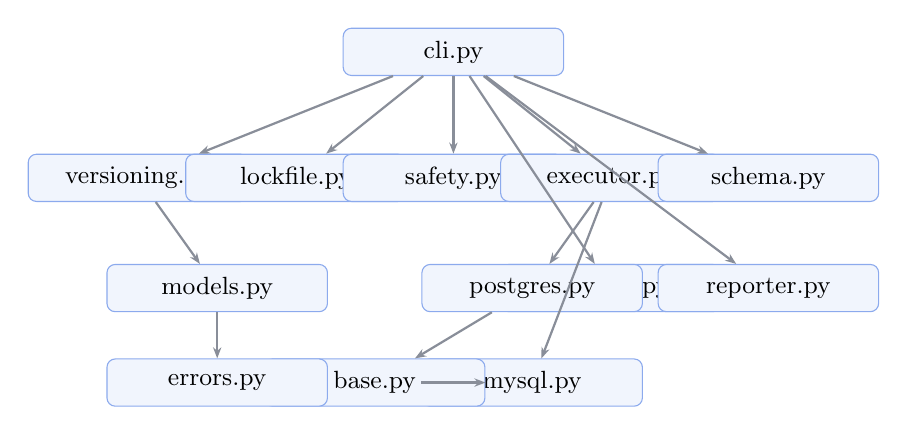
\begin{tikzpicture}[
  mod/.style={rectangle, rounded corners=3pt, draw=safeblue!50, fill=safeblue!6,
              minimum width=2.8cm, minimum height=0.6cm, font=\small},
  dep/.style={-{Stealth[length=4pt]}, thick, color=safegray!80},
  note/.style={font=\tiny\itshape, color=safegray}
]
  \node[mod] (cli)      at (4,0)    {cli.py};
  \node[mod] (ver)      at (0,-1.6) {versioning.py};
  \node[mod] (lock)     at (2,-1.6) {lockfile.py};
  \node[mod] (safe)     at (4,-1.6) {safety.py};
  \node[mod] (exec)     at (6,-1.6) {executor.py};
  \node[mod] (schema)   at (8,-1.6) {schema.py};
  \node[mod] (naming)   at (6,-3.0) {naming.py};
  \node[mod] (reporter) at (8,-3.0) {reporter.py};
  \node[mod] (pg)       at (5,-3.0) {postgres.py};
  \node[mod] (mysql)    at (5,-4.2) {mysql.py};
  \node[mod] (base)     at (3,-4.2) {base.py};
  \node[mod] (models)   at (1,-3.0) {models.py};
  \node[mod] (errors)   at (1,-4.2) {errors.py};

  \draw[dep] (cli) -- (ver);
  \draw[dep] (cli) -- (lock);
  \draw[dep] (cli) -- (safe);
  \draw[dep] (cli) -- (exec);
  \draw[dep] (cli) -- (schema);
  \draw[dep] (cli) -- (naming);
  \draw[dep] (cli) -- (reporter);
  \draw[dep] (exec) -- (pg);
  \draw[dep] (exec) -- (mysql);
  \draw[dep] (pg) -- (base);
  \draw[dep] (mysql) -- (base);
  \draw[dep] (ver) -- (models);
  \draw[dep] (models) -- (errors);
\end{tikzpicture}
\caption{Module dependency graph. \texttt{cli.py} is the sole orchestrator.}
\end{figure}

\section{The Adapter Pattern}

Both database adapters (\texttt{postgres.py} and \texttt{mysql.py}) implement the
abstract \texttt{DatabaseAdapter} base class defined in \texttt{adapters/base.py}:

\begin{lstlisting}[language=python, caption={DatabaseAdapter abstract interface}]
class DatabaseAdapter(ABC):
    @abstractmethod
    def execute_migrations(
        self,
        migrations: Iterable[Migration],
        dry_run: bool = False,
    ) -> None:
        pass
\end{lstlisting}

\noindent\textbf{Design rationale:} The \texttt{executor.py} orchestrator does
not import any DB-specific library. It only calls \texttt{adapter.execute\_migrations()}.
This allows a hypothetical SQLite or MSSQL adapter to be added without touching
any other file in the engine.

% ══════════════════════════════════════════════════════════════════════════════
\chapter{The Pipeline: Phase-by-Phase}
% ══════════════════════════════════════════════════════════════════════════════

\section{Phase 1 — Ordering (\texttt{versioning.py})}

\subsection{Purpose}

Before any SQL is read, SafeDB-CI validates that the migration files form a
\emph{complete, sequential, gap-free} sequence starting at version 001.

\subsection{Algorithm}

\begin{enumerate}
  \item Glob all \texttt{*.sql} files from the migrations directory.
  \item Extract the numeric prefix using the regex \texttt{r"\^(\textbackslash d+)\_"}.
  \item Sort by numeric prefix (not lexicographic string order).
  \item Walk the sorted list: if any version \( v_i \neq i \), raise
        \texttt{NonSequentialMigrationVersionError(expected=i, found=v\_i)}.
\end{enumerate}

\subsection{Design Decision: Why Strict Sequential Numbering?}

Permitting gaps (e.g.\ 001, 002, 004) makes migration history untrustworthy.
A gap is almost always a signal that someone deleted or renamed a file rather
than writing a proper compensating migration. Gaps that are ``allowed'' in
development accumulate and become impossible to reason about at scale.

\subsection{Error Produced}

\begin{lstlisting}
MIGRATION FAILED:
NonSequentialMigrationVersionError: Expected version 003, found 004.
Migration gap detected: file '004_create_orders.sql' follows '002_create_roles.sql'.
Write a '003_...' migration to fill the gap.
\end{lstlisting}

\section{Phase 1b — Tamper Detection (\texttt{lockfile.py})}

\subsection{Purpose}

After a successful run, SafeDB-CI records the SHA-256 hash of every migration
file in a JSON lockfile (\texttt{.safedb-lock}). On subsequent runs, any
modification to a previously-validated file is detected and treated as a hard
failure \emph{before} any database connection is opened.

\subsection{The \texttt{.safedb-lock} Format}

\begin{lstlisting}[language=json, caption={.safedb-lock example}]
{
  "safedb_version": "2.0.0",
  "last_validated": "2026-03-10T16:20:00+00:00",
  "migrations": {
    "001_create_users.sql":  "sha256:a3b4c5d6...",
    "002_create_roles.sql":  "sha256:f7e8d9c0...",
    "003_create_products.sql": "sha256:1a2b3c4d..."
  }
}
\end{lstlisting}

\subsection{Tamper Logic}

\begin{itemize}
  \item File in lockfile \textbf{and} hash matches: \textcolor{safegreen}{\textbf{PASS}}
  \item File in lockfile \textbf{and} hash differs: \textcolor{safered}{\textbf{TAMPER DETECTED}} (exit 1)
  \item File \textbf{not} in lockfile (new migration): \textcolor{safegreen}{\textbf{PASS}} (added on next success)
  \item File in lockfile but no longer on disk: ignored (ordering check catches missing files)
\end{itemize}

\subsection{Design Decision: Why Not Allow File Edits?}

Editing a committed migration is the most common cause of undetected schema drift.
Unlike a new migration, an edit changes a historical record without creating a
corresponding audit trail. The lockfile makes such edits impossible to deploy
silently.

\begin{infobox}{Commit the lockfile}
\texttt{.safedb-lock} should be committed to version control. It is not a cache —
it is the ground truth of what was last validated successfully.
\end{infobox}

\section{Phase 2 — Safety Scan (\texttt{safety.py})}

\subsection{Purpose}

Performs static analysis of every migration's SQL text \emph{before any
execution}. Detects destructive intent via regex pattern matching.

\subsection{Why Before Execution?}

The CI database is always empty. A \texttt{DROP TABLE users} will execute
successfully against an empty database but will destroy gigabytes of real data
in production. Static analysis catches destructive \emph{intent}, not just
runtime outcome.

\subsection{Rule Table}

\begin{center}
\begin{tabular}{@{}lll@{}}
\toprule
\textbf{Rule} & \textbf{Severity} & \textbf{Rationale} \\
\midrule
\texttt{DROP TABLE}               & HIGH   & Unconditional data destruction \\
\texttt{DROP COLUMN}              & HIGH   & Irreversible column removal \\
\texttt{TRUNCATE}                 & HIGH   & Unconditional table wipe \\
\texttt{ALTER TABLE … DROP}       & HIGH   & Dialect-agnostic column drop \\
\texttt{DELETE FROM <t>} (no WHERE) & HIGH & Full-table row deletion \\
\texttt{CASCADE}                  & MEDIUM & Conditional blast-radius amplifier \\
\texttt{ALTER COLUMN TYPE}        & MEDIUM & Silent data truncation risk \\
\texttt{ALTER COLUMN SET NOT NULL} & MEDIUM & Will fail on non-empty prod tables \\
\bottomrule
\end{tabular}
\end{center}

\subsection{Scanning Algorithm: The 3-Pass Line Processor}

\begin{enumerate}
  \item \textbf{Pass 1 — Allow detection:} Walk each line. If \texttt{-- safedb:allow}
        appears (inline or preceding line), mark that line (and the covered statement
        line) as allowed. Print an audit log entry for each override accepted.

  \item \textbf{Pass 2 — Comment stripping:} Blank out all allowed lines. Strip
        remaining \texttt{-- ...} comments from non-allowed lines.

  \item \textbf{Pass 3 — Regex scan:} Normalize whitespace. Run all rules against
        the cleaned SQL. Collect and report all violations at once.
\end{enumerate}

\subsection{The \texttt{safedb:allow} Override}

A destructive statement can be approved by a human reviewer using the annotation:

\begin{lstlisting}[language=sql, caption={safedb:allow annotation — two valid forms}]
-- Form 1: inline (recommended for single-statement approval)
DROP TABLE legacy_import_cache; -- safedb:allow

-- Form 2: preceding line (readable for documented operations)
-- safedb:allow
DROP TABLE old_events;
\end{lstlisting}

\textbf{Design constraints of the override:}
\begin{itemize}
  \item It is \textbf{per-line}. One annotation covers exactly one statement line.
  \item It is \textbf{always audited}. The CI log always contains
        \texttt{[SAFETY OVERRIDE]} entries — it cannot be silent.
  \item There is \textbf{no file-level override} by design — a \texttt{-- safedb:allow-file}
        would make it trivial to disable all scanning in a file accidentally.
\end{itemize}

\subsection{Severity Behaviour}

\begin{center}
\begin{tabular}{@{}lll@{}}
\toprule
 & \textbf{Default mode} & \textbf{--strict mode} \\
\midrule
HIGH violation  & Block (exit 1) & Block (exit 1) \\
MEDIUM violation & Warn (exit 0) & Block (exit 1) \\
\bottomrule
\end{tabular}
\end{center}

\section{Phase 3 — Execution (\texttt{executor.py} + adapters)}

\subsection{Purpose}

Applies all migrations to a live ephemeral database in sequence. Validates SQL
syntax, constraint definitions, and type compatibility at runtime.

\subsection{Normal Mode}

\begin{itemize}
  \item Each migration runs inside its own transaction (savepoint on Postgres).
  \item On failure: the failed migration's transaction is rolled back.
  \item The pipeline halts — subsequent migrations do not execute.
  \item The database contains all successfully-applied migrations up to the failure.
\end{itemize}

\subsection{Dry-Run Mode (\texttt{--dry-run})}

\begin{figure}[H]
\centering
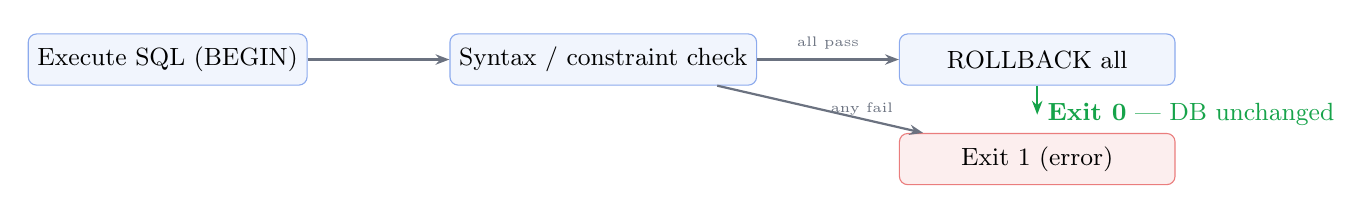
\begin{tikzpicture}[
  box/.style={rectangle, rounded corners=3pt, draw=safeblue!50, fill=safeblue!6,
              minimum width=3.5cm, minimum height=0.65cm, font=\small},
  arr/.style={-{Stealth[length=5pt]}, thick, color=safegray}
]
  \node[box] (exec)   {Execute SQL (BEGIN)};
  \node[box, right=1.8cm of exec] (check) {Syntax / constraint check};
  \node[box, right=1.8cm of check] (rb)  {ROLLBACK all};
  \node[box, below=0.6cm of rb, fill=safered!8, draw=safered!60] (fail) {Exit 1 (error)};
  \draw[arr] (exec) -- (check);
  \draw[arr] (check) -- node[above, font=\tiny]{all pass} (rb);
  \draw[arr] (check) -- node[right, font=\tiny]{any fail} (fail);
  \draw[arr,safegreen] (rb) -- ++(0,-0.7) node[right,font=\small,color=safegreen]
    {\textbf{Exit 0} — DB unchanged};
\end{tikzpicture}
\caption{Dry-run execution flow (Postgres only — full DDL rollback)}
\end{figure}

\begin{warningbox}{MySQL Dry-Run Limitation}
MySQL issues an implicit \texttt{COMMIT} before and after every DDL statement
(\texttt{CREATE TABLE}, \texttt{ALTER TABLE}, etc.). SafeDB-CI's \texttt{--dry-run}
rollback only affects DML statements in MySQL. For reliable dry-run, use PostgreSQL,
which supports fully transactional DDL.
\end{warningbox}

\subsection{Phases 4 and 5 Are Skipped in Dry-Run}

Because nothing was committed, the database catalog is unchanged. Opening an
introspection connection and running schema validation against it would be
meaningless. Phases 4, 5a, 5b, and 6 are marked \texttt{SKIPPED} in the report.

\section{Phase 4 — Schema Introspection (\texttt{schema.py})}

\subsection{Purpose}

After all migrations commit, SafeDB-CI opens a \emph{fresh read-only connection}
and queries the database catalog to build a \texttt{SchemaSnapshot} — a
normalized, in-memory representation of the resulting schema.

\subsection{Data Model}

\begin{lstlisting}[language=python, caption={SchemaSnapshot data model}]
@dataclass
class ColumnInfo:
    name: str
    data_type: str
    is_nullable: bool

@dataclass
class ForeignKeyInfo:
    constraint_name: str
    from_column: str   # source column in this table
    to_table: str      # referenced table
    to_column: str     # referenced column

@dataclass
class TableSchema:
    name: str
    columns: Dict[str, ColumnInfo]
    primary_key_columns: List[str]
    unique_constraint_columns: List[frozenset]
    foreign_keys: List[ForeignKeyInfo]

@dataclass
class SchemaSnapshot:
    tables: Dict[str, TableSchema]
\end{lstlisting}

\subsection{Why a Separate Connection?}

The \texttt{PostgresAdapter} uses psycopg's context manager, which closes its
connection on exit. The execution connection is gone by the time introspection
runs. Opening a fresh read connection is not overhead — it is the correct design.
It also means introspection always sees the committed state.

\subsection{Catalog Queries}

Both Postgres and MySQL implementations query \texttt{information\_schema}, which
provides a schema-agnostic SQL interface to column metadata, primary key membership,
unique constraints, and foreign key relationships. This keeps both implementations
readable and database-version-tolerant.

\section{Phase 5a — Structural Schema Validation (\texttt{schema.py})}

\subsection{Purpose}

Validates the internal \emph{relational self-consistency} of the schema. Execution
success ≠ structural correctness. This phase runs four checks:

\begin{center}
\begin{tabular}{@{}p{5.5cm}ll@{}}
\toprule
\textbf{Check} & \textbf{Severity} & \textbf{Why} \\
\midrule
FK references existing table    & HIGH   & Dangling FK = runtime constraint failures \\
FK references existing column   & HIGH   & Renamed/dropped column not updated \\
FK references PK or UNIQUE col  & HIGH   & Relational integrity requirement \\
Duplicate FK constraints        & MEDIUM & Write overhead + authoring error signal \\
Table missing PRIMARY KEY       & MEDIUM & Replication, ORM, and FK referencing issues \\
\bottomrule
\end{tabular}
\end{center}

\section{Phase 5b — Naming Heuristics (\texttt{naming.py})}

\subsection{Purpose}

Analyses column and table names for structural anti-patterns that suggest
normalization debt. These are \textbf{advisory} checks — always MEDIUM severity.

\subsection{Heuristic Rules}

\begin{center}
\begin{tabular}{@{}p{5cm}p{8cm}@{}}
\toprule
\textbf{Heuristic} & \textbf{Signal} \\
\midrule
Column named \texttt{*\_id} with no FK constraint &
  Developer likely forgot to declare the FK. \\
Junction table (name contains \texttt{\_}, has exactly 2 FKs) with no composite PK &
  Duplicate associations are possible without the PK. \\
Column named \texttt{*\_list}, \texttt{*\_csv}, \texttt{*\_ids}, \texttt{*\_array} &
  Likely storing multiple values in one field (1NF violation signal). \\
\bottomrule
\end{tabular}
\end{center}

\begin{infobox}{Heuristics Are Advisory}
Naming heuristics have known false-positive rates. A column named
\texttt{external\_id} is legitimately not a FK. The checks warn, not decide.
Use \texttt{--strict} to promote them to hard failures on production branches.
\end{infobox}

\section{Phase 6 — Lockfile Write (\texttt{lockfile.py})}

After all 8 phases complete successfully, SafeDB-CI writes (or updates) the
\texttt{.safedb-lock} file with the SHA-256 digest of every migration file.
The lockfile is only written on success — writing on failure would record a
broken state as the new baseline.

% ══════════════════════════════════════════════════════════════════════════════
\chapter{CLI Reference}
% ══════════════════════════════════════════════════════════════════════════════

\section{Invocation Syntax}

\begin{lstlisting}[language=bash]
safedb validate \
  --db-type   {postgres|mysql}  \
  --migrations-path PATH        \
  [--ci]                        \
  [--strict]                    \
  [--dry-run]                   \
  [--output {text|json}]        \
  [--lockfile-path PATH]        \
  [--database-url URL]          # postgres only, non-CI
\end{lstlisting}

\section{Argument Reference}

\begin{longtable}{@{}p{3.8cm}p{9cm}@{}}
\toprule
\textbf{Argument} & \textbf{Description} \\
\midrule
\endhead
\texttt{--db-type} &
  Target database engine. Required. \\
\texttt{--migrations-path} &
  Path to directory of numbered \texttt{***.sql} files. Required. \\
\texttt{--ci} &
  Read credentials from environment variables instead of CLI args.
  Postgres: \texttt{POSTGRES\_USER}, \texttt{POSTGRES\_PASSWORD}, \texttt{POSTGRES\_DB}.
  MySQL: \texttt{MYSQL\_USER}, \texttt{MYSQL\_PASSWORD}, \texttt{MYSQL\_DATABASE}. \\
\texttt{--strict} &
  Promote MEDIUM severity violations (safety, structural, naming) to hard failures. \\
\texttt{--dry-run} &
  Execute SQL inside \texttt{BEGIN}/\texttt{ROLLBACK}. Validates syntax without
  committing. Skips phases 4–6. PostgreSQL only for full rollback. \\
\texttt{--output \{text|json\}} &
  \texttt{text}: human-readable console output (default).
  \texttt{json}: writes \texttt{report.json} + GitHub Actions step summary. \\
\texttt{--lockfile-path} &
  Path to the lockfile (default: \texttt{.safedb-lock}).
  Should be committed to version control. \\
\texttt{--database-url} &
  Full PostgreSQL connection URL. Required when not using \texttt{--ci}
  with \texttt{--db-type postgres}. \\
\bottomrule
\end{longtable}

\section{Exit Codes}

\begin{center}
\begin{tabular}{@{}cl@{}}
\toprule
\textbf{Code} & \textbf{Meaning} \\
\midrule
0 & All phases passed \\
1 & Any phase failed (ordering, tamper, safety, execution, schema, naming) \\
\bottomrule
\end{tabular}
\end{center}

% ══════════════════════════════════════════════════════════════════════════════
\chapter{GitHub Actions Integration}
% ══════════════════════════════════════════════════════════════════════════════

\section{Composite Action (\texttt{action.yml})}

SafeDB-CI is packaged as a \textbf{composite action} — not a Docker action.
This offers two advantages:
\begin{itemize}
  \item No image build time on every use.
  \item Full access to the runner's checkout, secrets, and environment.
\end{itemize}

\subsection{Action Inputs}

\begin{center}
\begin{tabular}{@{}llp{6.5cm}@{}}
\toprule
\textbf{Input} & \textbf{Required} & \textbf{Description} \\
\midrule
\texttt{db\_type}           & Yes & \texttt{postgres} or \texttt{mysql} \\
\texttt{migrations\_path}   & Yes & Relative path to migrations directory \\
\texttt{strict\_mode}       & No  & \texttt{"true"} to enable \texttt{--strict} \\
\texttt{dry\_run}           & No  & \texttt{"true"} to enable \texttt{--dry-run} \\
\texttt{output\_format}     & No  & \texttt{text} (default) or \texttt{json} \\
\texttt{postgres\_user}     & No  & Required if \texttt{db\_type=postgres} \\
\texttt{postgres\_password} & No  & Required if \texttt{db\_type=postgres} \\
\texttt{postgres\_db}       & No  & Required if \texttt{db\_type=postgres} \\
\texttt{mysql\_user}        & No  & Required if \texttt{db\_type=mysql} \\
\texttt{mysql\_password}    & No  & Required if \texttt{db\_type=mysql} \\
\texttt{mysql\_database}    & No  & Required if \texttt{db\_type=mysql} \\
\bottomrule
\end{tabular}
\end{center}

\section{Example Workflow}

\begin{lstlisting}[language=yaml, caption={Minimal production workflow}]
name: SafeDB-CI Validate

on:
  push:
    branches: [main, release/**, feature/**]
  pull_request:
    branches: [main]

jobs:
  validate:
    runs-on: ubuntu-latest
    services:
      postgres:
        image: postgres:15
        env:
          POSTGRES_USER:     safedb
          POSTGRES_PASSWORD: ${{ secrets.DB_PASSWORD }}
          POSTGRES_DB:       safedb_test
        options: >-
          --health-cmd pg_isready
          --health-interval 10s
          --health-timeout 5s
          --health-retries 5

    steps:
      - uses: actions/checkout@v4

      - name: Run SafeDB-CI
        uses: arju-z/SafeDB-CI@v2
        with:
          db_type:          postgres
          migrations_path:  ./migrations
          strict_mode:      "true"
          output_format:    json
          postgres_user:    safedb
          postgres_password: ${{ secrets.DB_PASSWORD }}
          postgres_db:      safedb_test

      - name: Push to Loki
        if: always()
        run: |
          curl -X POST "${{ secrets.LOKI_URL }}/loki/api/v1/push" \
            -H "Content-Type: application/json" \
            -d "{\"streams\":[{
              \"stream\": {
                \"job\":       \"safedb-ci\",
                \"repo\":      \"${{ github.repository }}\",
                \"branch\":    \"${{ github.ref_name }}\",
                \"exit_code\": \"$(jq -r .exit_code report.json)\"
              },
              \"values\": [[\"$(date +%s%N)\", $(jq -c . report.json)]]
            }]}"
\end{lstlisting}

\section{Step Summary in GitHub Actions}

When \texttt{output\_format: json} is set, SafeDB-CI automatically writes a
Markdown table to \texttt{\$GITHUB\_STEP\_SUMMARY} when running inside GitHub
Actions. This renders directly in the PR check UI:

\begin{center}
\begin{tabular}{@{}llp{5cm}@{}}
\toprule
\textbf{Phase} & \textbf{Status} & \textbf{Detail} \\
\midrule
1. Ordering          & ✅ pass    & 3 migration(s) loaded \\
1b. Tamper Check     & ✅ pass    & All hashes match \\
2. Safety Scan       & ✅ pass    & — \\
3. Execution         & ✅ pass    & 3 migration(s) applied \\
4. Introspection     & ✅ pass    & 5 table(s) found \\
5a. Structural       & ✅ pass    & — \\
5b. Naming Heuristics & ⚠ warn    & 1 advisory warning \\
6. Lockfile          & ✅ pass    & 3 hashes recorded \\
\bottomrule
\end{tabular}
\end{center}

% ══════════════════════════════════════════════════════════════════════════════
\chapter{Observability Stack — Grafana / Loki}
% ══════════════════════════════════════════════════════════════════════════════

\section{Architecture}

\begin{figure}[H]
\centering
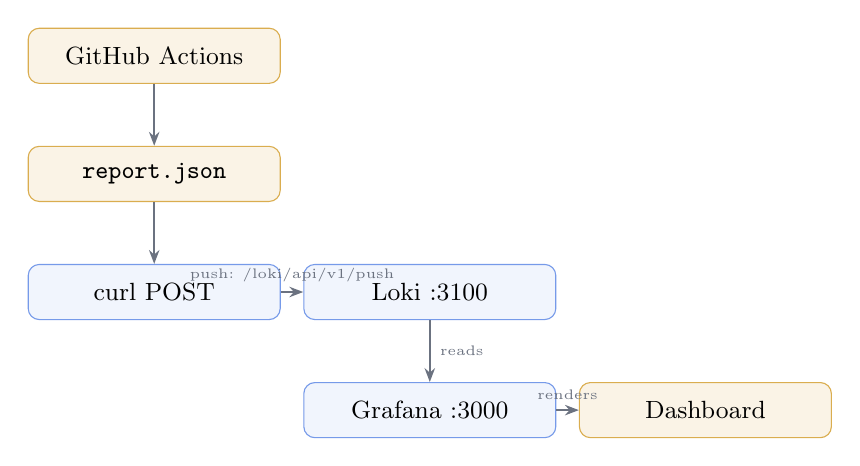
\begin{tikzpicture}[
  box/.style={rectangle, rounded corners=4pt, draw=safeblue!60, fill=safeblue!6,
              minimum width=3.2cm, minimum height=0.7cm, font=\small},
  ext/.style={box, fill=safeyellow!10, draw=safeyellow!70},
  arr/.style={-{Stealth[length=5pt]}, thick, color=safegray}
]
  \node[ext] (gh)     at (0, 0)    {GitHub Actions};
  \node[ext] (rj)     at (0,-1.5)  {\texttt{report.json}};
  \node[box] (curl)   at (0,-3.0)  {curl POST};
  \node[box] (loki)   at (3.5,-3.0){Loki :3100};
  \node[box] (graf)   at (3.5,-4.5){Grafana :3000};
  \node[ext] (browser)at (7,-4.5)  {Dashboard};

  \draw[arr] (gh) -- (rj);
  \draw[arr] (rj) -- (curl);
  \draw[arr] (curl) -- node[above,font=\tiny]{push: /loki/api/v1/push} (loki);
  \draw[arr] (loki) -- node[right,font=\tiny]{reads} (graf);
  \draw[arr] (graf) -- node[above,font=\tiny]{renders} (browser);
\end{tikzpicture}
\caption{Observability data flow. report.json is shipped to Loki via curl, then visualised in Grafana.}
\end{figure}

\section{Stack Startup}

\begin{lstlisting}[language=bash]
cd log
docker compose up -d
# Grafana: http://localhost:3000  (admin / safedb)
\end{lstlisting}

The \textbf{SafeDB-CI Migration Reports} dashboard is automatically provisioned
on startup. No manual configuration is required.

\section{Pre-built Dashboard Panels}

\begin{center}
\begin{tabular}{@{}p{4.5cm}p{8cm}@{}}
\toprule
\textbf{Panel} & \textbf{Description} \\
\midrule
Last Run Result &
  Stat panel — green (PASS) or red (FAIL) based on latest \texttt{exit\_code} label. \\
Total Runs &
  Count of all runs in the selected time range. \\
Failed Runs &
  Count with red threshold at $\geq 1$. \\
Raw JSON Reports &
  Log stream panel with prettified JSON, time-sorted descending. \\
Failed Run Details &
  Filtered log stream — only entries where \texttt{exit\_code=1}. \\
\bottomrule
\end{tabular}
\end{center}

\section{Useful LogQL Queries}

\begin{lstlisting}[caption={LogQL examples}]
# All CI runs
{job="safedb-ci"}

# Only failures
{job="safedb-ci", exit_code="1"}

# Filter by repository
{job="safedb-ci", repo="arju-z/SafeDB-CI"}

# Runs where safety phase failed
{job="safedb-ci"} | json | phases_safety_status = "fail"

# Failure rate over 7 days
count_over_time({job="safedb-ci", exit_code="1"}[7d])
  /
count_over_time({job="safedb-ci"}[7d])
\end{lstlisting}

\section{Exposing Loki to GitHub Actions Runners}

GitHub-hosted runners run on ephemeral cloud VMs. Three approaches to connect them
to your Loki instance:

\begin{enumerate}
  \item \textbf{ngrok} — Fastest for local testing:
        \texttt{ngrok http 3100}, set the forwarding URL as \texttt{LOKI\_URL} secret.
  \item \textbf{Public VPS} — Deploy the \texttt{log/} stack on any cloud server.
        Open port 3100 in the firewall, set the public IP as \texttt{LOKI\_URL}.
  \item \textbf{Tailscale} — Use the
        \href{https://github.com/tailscale/github-action}{Tailscale GitHub Action}
        to connect runners to your private network without opening ports.
\end{enumerate}

% ══════════════════════════════════════════════════════════════════════════════
\chapter{Test Scenarios}
% ══════════════════════════════════════════════════════════════════════════════

Eight example scenario directories cover every branch of the pipeline:

\begin{longtable}{@{}p{5cm}p{3cm}p{5cm}@{}}
\toprule
\textbf{Scenario} & \textbf{Exit Code} & \textbf{Failing Phase} \\
\midrule
\endhead
\texttt{01\_clean\_pass}         & 0 & None — all phases pass \\
\texttt{02\_safety\_blocked}     & 1 & Phase 2 (HIGH: DROP TABLE, TRUNCATE, DELETE) \\
\texttt{03\_schema\_integrity\_fail} & 1 & Phase 5a (tables with no PRIMARY KEY) \\
\texttt{04\_ordering\_fail}      & 1 & Phase 1 (version 003 missing, 004 present) \\
\texttt{05\_execution\_fail}     & 1 & Phase 3 (SQL syntax error in migration 002) \\
\texttt{06\_naming\_warnings}    & 0 (warn) / 1 (strict) & Phase 5b (orphaned \_id, array column, junction PK) \\
\texttt{07\_dry\_run}            & 0 & None — dry-run validates, rolls back \\
\texttt{08\_safety\_override}    & 0 & Phase 2 passed via safedb:allow annotation \\
\bottomrule
\end{longtable}

\section{Running Scenarios Locally}

\begin{lstlisting}[language=bash]
# Pre-requisite: Postgres running, env vars exported
export POSTGRES_USER=safedb POSTGRES_PASSWORD=safedbpass POSTGRES_DB=safedb_test

# Scenario 1 — should exit 0
safedb validate --db-type postgres --ci \
  --migrations-path ./examples/01_clean_pass

# Scenario 2 — should exit 1 (safety blocked)
safedb validate --db-type postgres --ci \
  --migrations-path ./examples/02_safety_blocked

# Scenario 6 — warnings only (exit 0)
safedb validate --db-type postgres --ci \
  --migrations-path ./examples/06_naming_warnings

# Scenario 6 — strict mode (exit 1)
safedb validate --db-type postgres --ci --strict \
  --migrations-path ./examples/06_naming_warnings

# Scenario 7 — dry-run (run twice: DB always clean)
safedb validate --db-type postgres --ci --dry-run \
  --migrations-path ./examples/07_dry_run

# Scenario 8 — safedb:allow override (exit 0)
safedb validate --db-type postgres --ci \
  --migrations-path ./examples/08_safety_override

# JSON output with GHA summary
safedb validate --db-type postgres --ci --output json \
  --migrations-path ./migrations
cat report.json | jq .
\end{lstlisting}

% ══════════════════════════════════════════════════════════════════════════════
\chapter{Design Options and Alternatives Considered}
% ══════════════════════════════════════════════════════════════════════════════

\section{Why Regex Safety Scanning (Not a SQL Parser)?}

\begin{center}
\begin{tabular}{@{}p{5cm}p{4.5cm}p{4.5cm}@{}}
\toprule
& \textbf{Regex (chosen)} & \textbf{SQL Parser (rejected)} \\
\midrule
Dependencies    & None (stdlib \texttt{re}) & sqlparse, antlr, pglast \\
Dialect support & Universal (case-insensitive) & Per-dialect, diverging APIs \\
Maintenance     & Rules are auditable strings & AST traversal, fragile \\
False positives & Known, documented & Fewer, but harder to debug \\
Speed           & Sub-millisecond & Potential startup overhead \\
\bottomrule
\end{tabular}
\end{center}

\textbf{Verdict:} For \emph{intent detection} (not syntax validation), regex is
the pragmatic choice. Syntax validation is already performed by the database
engine in Phase 3.

\section{Why Composite Action (Not Docker)?}

\begin{center}
\begin{tabular}{@{}p{5cm}p{4.5cm}p{4.5cm}@{}}
\toprule
& \textbf{Composite (chosen)} & \textbf{Docker (rejected)} \\
\midrule
Cold start time & Seconds (pip install) & Minutes (image pull) \\
Arch support    & arm64, x86\_64 automatic & Must multi-platform build \\
Secret access   & Full runner env access & Passed explicitly via \texttt{-e} \\
Debugging       & Runner logs directly & Requires container log access \\
\bottomrule
\end{tabular}
\end{center}

\section{Why Loki + Grafana (Not ELK)?}

\begin{center}
\begin{tabular}{@{}p{5cm}p{4.5cm}p{4.5cm}@{}}
\toprule
& \textbf{Loki + Grafana} & \textbf{Elasticsearch + Kibana} \\
\midrule
Memory footprint & $\sim$256MB total & $\sim$2GB+ for ES alone \\
Push protocol   & Simple HTTP POST + JSON & Requires Logstash / Filebeat \\
Index model     & Label-based (no full-text index) & Full inverted index \\
JSON query      & LogQL \texttt{| json} & Full-text KQL / Lucene \\
License         & Apache 2.0 & SSPL (partially proprietary) \\
\bottomrule
\end{tabular}
\end{center}

\textbf{Verdict:} For structured CI log ingest with simple label queries,
Loki is dramatically lighter and simpler than the ELK stack.

\section{Normalization Warnings: Why Not 1NF/2NF/3NF/BCNF?}

During v2 planning, full normal form analysis was considered. It was rejected for
these reasons:

\begin{itemize}
  \item Normalization to 2NF, 3NF, and BCNF requires \emph{knowledge of functional
        dependencies} — which column determines which other column.
  \item Functional dependencies are a semantic concept. They cannot be inferred
        from column names, data types, or constraint definitions alone.
  \item No database catalog stores functional dependencies. They exist only in the
        application's domain model.
  \item A heuristic approach (naming patterns, structural anti-patterns) can detect
        the \emph{most common} normalization mistakes without requiring mathematical
        FD analysis.
\end{itemize}

The chosen approach (Phase 5b naming heuristics) catches the real-world cases that
matter most — forgotten FKs, junction tables without PKs, CSV columns — without
the complexity or false confidence of attempting formal BCNF checking.

% ══════════════════════════════════════════════════════════════════════════════
\chapter{Security Model}
% ══════════════════════════════════════════════════════════════════════════════

\section{Credential Handling}

\begin{itemize}
  \item Credentials are \textbf{never} passed as CLI positional arguments (which
        appear in process listings and shell history).
  \item In \texttt{--ci} mode, credentials are read from environment variables
        that GitHub Actions injects from encrypted secrets.
  \item The connection URL is constructed in memory, never written to disk or logs.
\end{itemize}

\section{Tamper Model}

The lockfile provides ground-truth integrity for committed migration files.
Attack scenarios it protects against:

\begin{enumerate}
  \item Developer silently edits a committed migration to fix a bug
        (changes history without audit trail).
  \item Automated tooling accidentally overwrites migration files during
        code generation.
  \item CI configuration change causes migrations to be served from a
        different directory (path mismatch would cause new hashes).
\end{enumerate}

\section{Safety Override Audit Trail}

Every \texttt{safedb:allow} override is logged to CI stdout as:

\begin{lstlisting}
[SAFETY OVERRIDE] 001_replace_legacy_users.sql:42: safedb:allow —
  reviewer override accepted for: 'DROP TABLE IF EXISTS legacy_user_accounts;'
\end{lstlisting}

This line appears in the GitHub Actions log, which is immutable and retained per
the repository's log retention policy. The override cannot be silent.

% ══════════════════════════════════════════════════════════════════════════════
\chapter{Known Limitations and Future Work}
% ══════════════════════════════════════════════════════════════════════════════

\section{Known Limitations}

\begin{enumerate}
  \item \textbf{Empty CI database:} The CI database is always empty. Data-level
        validation (e.g.\ detecting SET NOT NULL failures due to existing NULLs)
        is impossible without a production snapshot.

  \item \textbf{Public schema only (PostgreSQL):} All introspection queries
        filter to \texttt{table\_schema = 'public'}. Multi-schema PostgreSQL databases
        are not supported.

  \item \textbf{Multi-statement migrations:} The MySQL adapter splits on \texttt{;},
        which can break stored procedures and triggers that use \texttt{DELIMITER}.

  \item \textbf{Naming heuristic false positives:} A column named
        \texttt{external\_id} is legitimately not a FK. A table named
        \texttt{user\_settings} with 2 FKs might be a configuration table, not a
        junction table. Heuristics are advisory by design.

  \item \textbf{safedb:allow is line-level only:} Multi-line destructive
        statements (rare in practice) require an annotation on the first line.
        The current implementation does not span block detection.
\end{enumerate}

\section{Potential Future Work}

\begin{itemize}
  \item \textbf{SQLite adapter} — Zero-dependency local-only validation for library projects.
  \item \textbf{Rollback plan generation} — Auto-generate a compensating migration
        when a destructive operation is detected.
  \item \textbf{Schema diffing} — Compare the resulting schema against a pinned
        \texttt{schema.json} baseline for drift detection.
  \item \textbf{Parallel scenario testing} — Run multiple \texttt{examples/}
        scenarios in parallel in CI using a job matrix.
  \item \textbf{Grafana alerting} — Pre-wire Grafana alert rules to notify on
        consecutive failures on the main branch.
\end{itemize}

% ──────────────────────────────────────────────────────────────────────────────
\appendix
% ──────────────────────────────────────────────────────────────────────────────

\chapter{JSON Report Schema}

\begin{lstlisting}[language=json, caption={report.json full schema}]
{
  "safedb_version": "2.0.0",
  "db_type":        "postgres",
  "migrations_path": "./migrations",
  "dry_run":        false,
  "exit_code":      0,
  "timestamp":      "2026-03-10T16:20:00+00:00",
  "phases": {
    "ordering":  { "status": "pass", "detail": "6 migration(s) loaded" },
    "tamper_check": { "status": "pass", "detail": "All hashes match" },
    "safety":    { "status": "pass" },
    "execution": { "status": "pass", "detail": "6 migration(s) applied" },
    "introspection": { "status": "pass", "detail": "8 table(s) found" },
    "structural_validation": { "status": "pass" },
    "naming_heuristics": { "status": "pass" },
    "lockfile":  { "status": "pass", "detail": "6 hashes recorded" }
  }
}
\end{lstlisting}

\chapter{Migration File Naming Convention}

\begin{itemize}
  \item Format: \texttt{NNN\_description.sql} where \texttt{NNN} is zero-padded.
  \item Examples: \texttt{001\_create\_users.sql}, \texttt{042\_add\_index\_on\_email.sql}
  \item The prefix must be sequential with no gaps from 001.
  \item The description is free-form (lowercase, underscores recommended).
  \item Files not matching the pattern are silently ignored.
\end{itemize}

\chapter{Environment Variable Reference}

\begin{center}
\begin{tabular}{@{}lll@{}}
\toprule
\textbf{Variable}        & \textbf{DB}   & \textbf{Used in \texttt{--ci} mode} \\
\midrule
\texttt{POSTGRES\_USER}     & PostgreSQL & ✅ \\
\texttt{POSTGRES\_PASSWORD} & PostgreSQL & ✅ \\
\texttt{POSTGRES\_DB}       & PostgreSQL & ✅ \\
\texttt{MYSQL\_USER}        & MySQL      & ✅ \\
\texttt{MYSQL\_PASSWORD}    & MySQL      & ✅ \\
\texttt{MYSQL\_DATABASE}    & MySQL      & ✅ \\
\texttt{GITHUB\_STEP\_SUMMARY} & — & Auto-detected for step summary writing \\
\texttt{LOKI\_URL}          & — & Used in workflow Loki push step \\
\bottomrule
\end{tabular}
\end{center}

\end{document}
